% !TEX root = ../../Tesi.tex

%******************************************
%	Resoconto dello stage
%******************************************

\chapter{Resoconto dello stage}
\label{cap:resoconto_dello_stage}

	\section{Individuazione dei motori di ricerca}
	Ad oggi, sono disponibili in rete un gran numero di motori di ricerca, sia proprietari, sia \gls{open source}. Questi, mettono a disposizione funzionalità di ricerca più o meno avanzate e, a seconda di vari fattori come possono essere, ad esempio, la tipologia e la quantità di dati che vogliamo indicizzare, rendendoli ricercabili agli utenti, possiamo optare per l'uno piuttosto che per l'altro. \\
	La scelta del motore di ricerca più adatto alle specifiche esigenze, non è questione affatto banale; molte volte esistono varie soluzioni in grado di modellare bene il problema che dobbiamo affrontare, simili tra loro, che differiscono però per alcuni aspetti chiave. \\
	Focalizzando l'attenzione sulle esigenze dettate dai siti informativi Camerali, possiamo già applicare un primo filtro sui motori di ricerca da utilizzare: motori di ricerca proprietari \textit{vs} motori di ricerca \gls{open source}. \\
	Un motore di ricerca proprietario rappresenta indubbiamente un onere per l'azienda e, oltre a ciò, quest'ultima non ha il pieno controllo sulla destinazione finale dei dati; queste questioni non si hanno invece in un sistema \gls{open source}, nel quale il codice sorgente è liberamente modificabile e analizzabile, avendo dunque il pieno controllo sull'intero sistema. \\
	Nella figura 3.1 è presente una classifica dei motori di ricerca, aggiornata a Novembre 2017, calcolata su parametri che rappresentano la popolarità del sito (maggiori informazioni sui punteggi assegnati sono disponili al seguente indirizzo: \url{https://db-engines.com/en/ranking_definition}). Da questa tabella, notiamo come in testa alla classifica siano presenti tre motori di ricerca che hanno un ampio margine di distacco, in termini di punteggio ad essi attribuito, rispetto alle tecnologie che li precedono. Di questi, solamente i primi due (\gls{Solr} e \gls{ElasticSearch}) sono alternative \gls{open source}. \\
	Oltre a ciò, per entrambi i motori di ricerca appena citati, sono disponibili \glspl{Modulo} \gls{Drupal} che rendono possibile la semplice integrazione tra i motori di ricerca e il \gls{CMSg} di interesse. \\
	Le motivazioni appena descritte, hanno così portato alla selezione di \gls{Solr} e \gls{ElasticSearch} come motori di ricerca da studiare nell'ambito dello stage.

	\begin{figure}[htbp]
		\begin{center}
			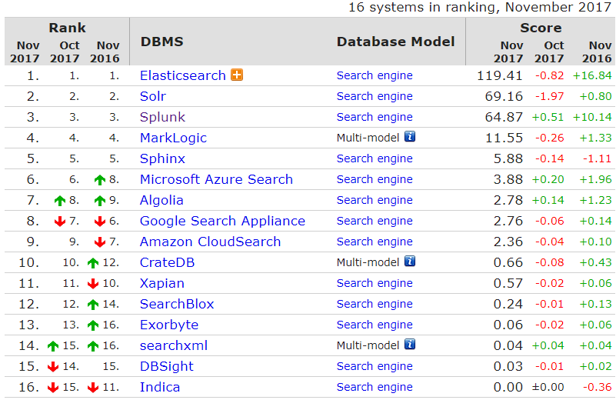
\includegraphics[width=13cm]{tabella_SE}
			\captionof{figure}{\cite{site:confronto_SE}}
		\end{center}
	\end{figure}
	
	\section{Pianificazione}
	Durante la stesura del Piano di Lavoro, assieme al tutor aziendale, ho concordato le attività principali da svolgere durante il periodo di stage, della durata di circa 300 ore, previsto dal mio corso di laurea. Nel documento sopracitato, sono inoltre contenute le \gls{Milestone} pianificate, così come descritto nella \hyperref[subsub:milestone]{sezione 2.2.2, sotto alla voce "Le milestone"}. \\
	Oltre al resoconto quotidiano con il tutor aziendale, al completamento di ogni attività, abbiamo fatto il punto della situazione sullo stato di avanzamento del lavoro, rivedendo e integrando, quando necessario, gli obiettivi settimanali previsti dal Piano di Lavoro. Questa modalità di operare mi ha permesso di rispettare le attività pianificate fin dall'inizio, oltre ad ampliare lo studio delle funzionalità di ricerca offerte da \gls{Drupal}, non inizialmente previste, necessarie però a fornire un quadro più dettagliato sull'intero ambito di lavoro.
	Nell'ultima settimana lavorativa, l'azienda ha inoltre richiesto una presentazione, esposta verbalmente e corredata da diapositive illustrative, sul lavoro operato durante lo stage e sulle relative conclusioni. Più nel dettaglio, nella presentazione ho presentato: scopo e motivazioni del lavoro svolto; come ho organizzato il mio lavoro; funzionalità offerte dalle tecnologie da me esaminate (di interesse per l'azienda); conclusione soggettiva su quale tecnologia sia più adatta nell'ambito dei siti camerali, con suggerimenti per migliorare le funzionalità di ricerca dei suddetti siti; benefici immediati e a lungo termine che il lavoro svolto durante lo stage ha apportato all'azienda; ulteriori ambiti da esplorare, relativamente a queste tecnologie; valutazione soggettiva, mia e del tutor aziendale, riguardo allo stage come esperienza. \\
	
	\section{I siti istituzionali delle Camere di Commercio}

		\subsection{Funzionalità di ricerca attuali}
		Questa sezione presenterà la struttura dei siti camerali attualmente in produzione, ponendo l'accento sugli strumenti messi a disposizione all'utente per ritrovare i contenuti in esso presenti.
		
		\begin{figure}[htbp]
			\begin{center}
				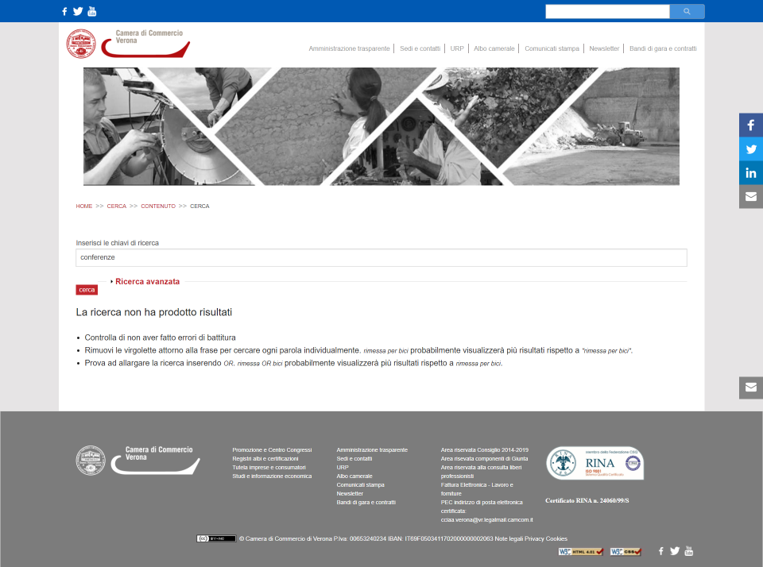
\includegraphics[width=13cm]{vr_attuale}
				\captionof{figure}{\cite{site:vr_attuale}}
			\end{center}
		\end{figure}
		
		
		\subsection{Possibile evoluzione}
		Questa sezione presenterà una possibile evoluzione dei siti camerali, contenente funzionalità di ricerca attualmente non presenti.
		
		\begin{figure}[htbp]
			\begin{center}
				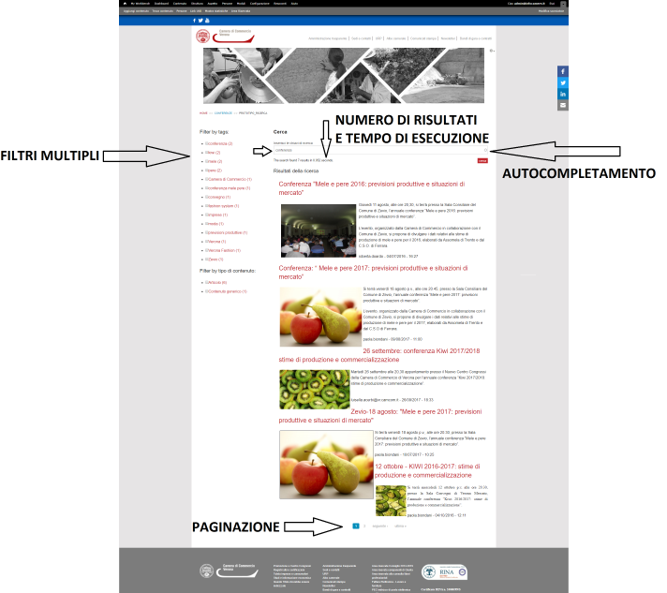
\includegraphics[width=13cm]{vr_futura}
				\captionof{figure}{Possibile evoluzione, mediante aggiunta di funzionalità di ricerca, del sito informativo Camerale di Verona}
			\end{center}
		\end{figure}

	\section{Ricerca nativa Drupal}

		\subsection{Introduzione a Drupal}
		Qui verrà introdotto Drupal, spiegando cos'è e come funziona.
		
		\subsection{Ricerca di base e avanzata}
		Qui verranno presentate le principali funzionalità offerte dalla prima tipologia di ricerca nativa Drupal.
		
		\subsection{Ricerca con Search API}
		Qui verranno presentate le principali funzionalità offerte dalla seconda tipologia di ricerca nativa Drupal.
		
		\subsection{Considerazioni di Drupal nativo}
		Questa sezione conterrà conclusioni riguardanti le funzionalità di ricerca offerte globalmente dalla ricerca nativa Drupal.

	\section{Ricerca con Solr}

		\subsection{Introduzione a Solr}
		Qui verrà introdotto Solr, spiegando cos'è e come funziona.
		%Ranking
		
		\subsection{Principali funzionalità di ricerca}
		Qui verranno presentate le principali funzionalità di ricerca offerte dal motore di ricerca Solr, di possibile interesse per i siti camerali.
			
		\subsection{Integrazione con Drupal}
		Qui verranno discusse le funzionalità di ricerca derivanti dall'integrazione tra Solr e Drupal.
			
			\subsubsection{Apache Solr}
			Qui verranno discusse le funzionalità di ricerca derivanti dall'integrazione tra Solr e Drupal mediante il modulo Apache Solr Search.
			
			\subsubsection{Search API Solr}
			Qui verranno discusse le funzionalità di ricerca derivanti dall'integrazione tra Solr e Drupal mediante il modulo Search API Solr Search.
	
	\section{Ricerca con ElasticSearch}
	
		\subsection{Introduzione a ElasticSearch}
		Qui verrà introdotto ElasticSearch, spiegando cos'è e come funziona.
		%Ranking

		\subsection{Principali funzionalità di ricerca}
		Qui verranno presentate le principali funzionalità di ricerca offerte dal motore di ricerca ElasticSearch, di possibile interesse per i siti camerali.
		
		\subsection{Integrazione con Drupal}
		Qui verranno discusse le funzionalità di ricerca derivanti dall'integrazione tra ElasticSearch e Drupal.
		%Accenno alla versione Drupal8?
		
			\subsubsection{Search API ElasticSearch}
			Qui verranno discusse le funzionalità di ricerca derivanti dall'integrazione tra ElasticSearch e Drupal mediante il modulo Search API ElasticSearch.
			
	\section{Considerazioni finali sui motori di ricerca esaminati}
	Questa sezione conterrà un confronto tra le principali funzionalità, possibilmente di interesse per l'azienda, offerte dalle tecnologie esaminate e quale di queste potrebbe essere la più adatta ai siti camerali.